\documentclass[svgnames,11pt]{beamer}
\input{/home/tof/Documents/Cozy/latex-include/preambule_commun.tex}
\input{/home/tof/Documents/Cozy/latex-include/preambule_beamer.tex}
%\usepackage{pgfpages} \setbeameroption{show notes on second screen=left}
\author[]{Christophe Viroulaud}
\title{Arbre binaire\\Notation polonaise}
\date{\framebox{\textbf{Algo 06}}}
%\logo{}
\institute{Terminale - NSI}

\begin{document}
\begin{frame}
    \titlepage
\end{frame}
\begin{frame}
    \frametitle{}
    En 1920 le mathématicien Jan Łukasiewicz présente la \emph{notation polonaise} qui permet d'exprimer des expressions mathématiques sans utiliser de parenthèse, mais traitant néanmoins toute formule sans ambiguïté.\\
    L'expression arithmétique
    $$2~×~(3+4)$$
    devient en notation polonaise
    $$×~2+3~4$$


\end{frame}
\begin{frame}
    \frametitle{}

    Dans les années 50, Charles L. Hamblin s'intéresse à variante \emph{inversée} de cette notation. Elle est en effet particulièrement bien adaptée à la manière dont les processeurs traitent leurs opérandes.
    En notation polonaise inversée, l'expression précédente s'écrit
    $$2~3~4~+~×$$
    \note{En 1972 Hewlett-Packard sort une calculatrice financière en notation polonaise inversée = gain de temps car moins de touches à utiliser}
\end{frame}
\begin{frame}
    \frametitle{}

    \begin{framed}
        Déterminer une structure de données adaptée au calcul en notation polonaise inversée.
    \end{framed}

\end{frame}
\section{Arbre binaire}
\subsection{Définition}
\begin{frame}
    \frametitle{Arbre binaire - définition}
    \begin{aretenir}[]
        Un \textbf{arbre binaire} est une structure arborescente où chaque nœud possède \textbf{au plus} deux fils. L'ordre des nœuds-fils est pris en compte: on parle alors de fils \emph{gauche} et fils \emph{droit}.
    \end{aretenir}
    \begin{center}
        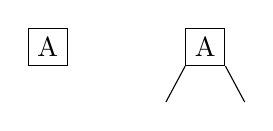
\begin{tikzpicture}
            \node[draw] (A) at (0,0) {A};
            \node[draw] (B) at (2,0) {A};

            \draw (B.south west) -- (1.5,-0.7);
            \draw (B.south east) -- (2.5,-0.7);
        \end{tikzpicture}
        \captionof{figure}{Représentations d'un nœud}
        \label{noeud}
    \end{center}

\end{frame}
\begin{frame}
    \frametitle{}

    \begin{center}
        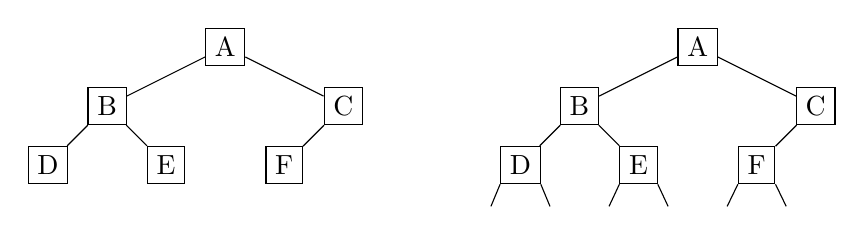
\begin{tikzpicture}[scale=0.75]
            \node[draw] (A) at (-3,0) {A};
            \node[draw] (B) at (-5,-1) {B};
            \node[draw] (C) at (-1,-1) {C};
            \node[draw] (D) at (-6,-2) {D};
            \node[draw] (E) at (-4,-2) {E};
            \node[draw] (F) at (-2,-2) {F};

            \draw (A) -- (B);
            \draw (A) -- (C);
            \draw (B) -- (D);
            \draw (B) -- (E);
            \draw (C) -- (F);

            \node[draw] (A1) at (5,0) {A};
            \node[draw] (B1) at (3,-1) {B};
            \node[draw] (C1) at (7,-1) {C};
            \node[draw] (D1) at (2,-2) {D};
            \node[draw] (E1) at (4,-2) {E};
            \node[draw] (F1) at (6,-2) {F};

            \draw (A1) -- (B1);
            \draw (A1) -- (C1);
            \draw (B1) -- (D1);
            \draw (B1) -- (E1);
            \draw (C1) -- (F1);
            \draw (D1.south west) -- (1.5,-2.7);
            \draw (D1.south east) -- (2.5,-2.7);
            \draw (E1.south west) -- (3.5,-2.7);
            \draw (E1.south east) -- (4.5,-2.7);
            \draw (F1.south west) -- (5.5,-2.7);
            \draw (F1.south east) -- (6.5,-2.7);
        \end{tikzpicture}
        \captionof{figure}{Représentations d'un arbre binaire}
        \label{arbre}
    \end{center}

\end{frame}
\subsection{vocabulaire}
\begin{frame}
    \frametitle{vocabulaire}

    \begin{aretenir}[]
        Un arbre binaire est \textbf{complet} si tous les niveaux sont remplis sauf éventuellement le dernier; les feuilles sont alors \emph{tassées à gauche}
    \end{aretenir}
    \begin{center}
        \begin{tikzpicture}
            \node[draw] (A) at (0,0) {A};
            \node[draw] (B) at (-3,-1) {B};
            \node[draw] (C) at (-5,-2) {C};
            \node[draw] (D) at (-1,-2) {D};
            \node[draw] (E) at (-6,-3) {E};
            \node[draw] (F) at (-4,-3) {F};
            \node[draw] (H) at (-2,-3) {H};
            \node[draw] (I) at (3,-1) {I};
            \node[draw] (J) at (2,-2) {J};
            \node[draw] (K) at (4,-2) {K};
            \node[draw] (L) at (0,-3) {L};
            \draw (A) -- (B);
            \draw (C) -- (B);
            \draw (C) -- (E);
            \draw (C) -- (F);
            \draw (D) -- (B);
            \draw (D) -- (H);
            \draw (A) -- (I);
            \draw (J) -- (I);
            \draw (I) -- (K);
            \draw (L) -- (D);
        \end{tikzpicture}
        \captionof{figure}{Un arbre binaire complet}
        \label{arbre}
    \end{center}
\end{frame}
\begin{frame}
    \frametitle{}

    \begin{aretenir}[]
        Un arbre binaire est \textbf{équilibré} si pour chaque nœud interne, les \emph{sous-arbres gauche et droite} ont une hauteur qui diffère au plus de 1.
    \end{aretenir}
    \begin{center}
        \begin{tikzpicture}
            \node[draw] (A) at (0,0) {A};
            \node[draw] (B) at (-3,-1) {B};
            \node[draw] (C) at (-5,-2) {C};
            \node[draw] (D) at (-1,-2) {D};
            \node[draw] (E) at (-6,-3) {E};
            \node[draw] (F) at (-4,-3) {F};
            \node[draw] (H) at (-2,-3) {H};
            \node[draw] (I) at (3,-1) {I};
            \node[draw] (J) at (2,-2) {J};
            \node[draw] (K) at (4,-2) {K};
            \node[draw] (L) at (5,-3) {L};
            \draw (A) -- (B);
            \draw (C) -- (B);
            \draw (C) -- (E);
            \draw (C) -- (F);
            \draw (D) -- (B);
            \draw (D) -- (H);
            \draw (A) -- (I);
            \draw (J) -- (I);
            \draw (I) -- (K);
            \draw (L) -- (K);
        \end{tikzpicture}
        \captionof{figure}{Un arbre binaire équilibré non complet}
        \label{arbre}
    \end{center}
\end{frame}
\begin{frame}
    \frametitle{}

    \begin{aretenir}[]
        Un arbre binaire est \textbf{parfait} si tous les niveaux sont remplis.
    \end{aretenir}
    \begin{center}
        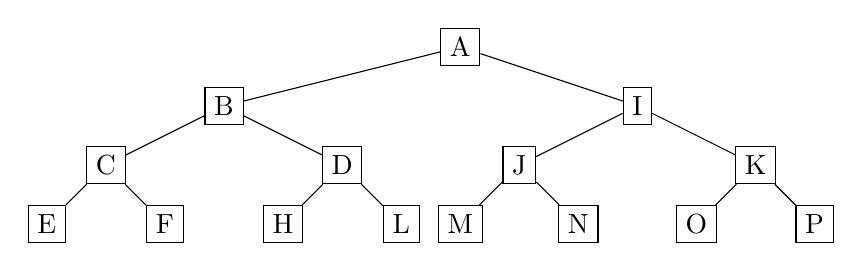
\begin{tikzpicture}[scale=0.75]
            \node[draw] (A) at (1,0) {A};
            \node[draw] (B) at (-3,-1) {B};
            \node[draw] (C) at (-5,-2) {C};
            \node[draw] (D) at (-1,-2) {D};
            \node[draw] (E) at (-6,-3) {E};
            \node[draw] (F) at (-4,-3) {F};
            \node[draw] (H) at (-2,-3) {H};
            \node[draw] (I) at (4,-1) {I};
            \node[draw] (J) at (2,-2) {J};
            \node[draw] (K) at (6,-2) {K};
            \node[draw] (L) at (0,-3) {L};
            \node[draw] (M) at (1,-3) {M};
            \node[draw] (N) at (3,-3) {N};
            \node[draw] (O) at (5,-3) {O};
            \node[draw] (P) at (7,-3) {P};

            \draw (A) -- (B);
            \draw (C) -- (B);
            \draw (C) -- (E);
            \draw (C) -- (F);
            \draw (D) -- (B);
            \draw (D) -- (H);
            \draw (A) -- (I);
            \draw (J) -- (I);
            \draw (I) -- (K);
            \draw (L) -- (D);
            \draw (J) -- (M);
            \draw (J) -- (N);
            \draw (K) -- (O);
            \draw (K) -- (P);
        \end{tikzpicture}
        \captionof{figure}{Un arbre binaire parfait}
        \label{arbre}
    \end{center}
\end{frame}

\subsection{Propriétés}
\begin{frame}
    \frametitle{Propriétés}
    \begin{aretenir}[]
        Dans un arbre binaire, la taille \emph{N} et la hauteur \emph{h} sont liées par les inégalités:
        \begin{center}
            $h+1 \leqslant N \leqslant 2^{h+1}-1$
        \end{center}
    \end{aretenir}
    \begin{center}
        \begin{tikzpicture}
            \node[draw] (A) at (0,0) {A};
            \node[draw] (B) at (-3,-1) {B};
            \node[draw] (C) at (-5,-2) {C};
            \node[draw] (D) at (-1,-2) {D};
            \node[draw] (E) at (-6,-3) {E};
            \node[draw] (F) at (-4,-3) {F};
            \node[draw] (H) at (-2,-3) {H};
            \node[draw] (I) at (3,-1) {I};
            \node[draw] (J) at (2,-2) {J};
            \node[draw] (K) at (4,-2) {K};
            \node[draw] (L) at (0,-3) {L};
            \draw (A) -- (B);
            \draw (C) -- (B);
            \draw (C) -- (E);
            \draw (C) -- (F);
            \draw (D) -- (B);
            \draw (D) -- (H);
            \draw (A) -- (I);
            \draw (J) -- (I);
            \draw (I) -- (K);
            \draw (L) -- (D);
        \end{tikzpicture}
        \captionof{figure}{Un arbre binaire complet}
        \label{arbre}
    \end{center}

\end{frame}
\begin{frame}
    \frametitle{Démonstration}

    \begin{center}
        \begin{tikzpicture}
            \node[draw] (A) at (0,0) {A};
            \node[draw] (B) at (-1,-1) {B};
            \node[draw] (C) at (-2,-2) {C};
            \node[draw] (D) at (-3,-3) {D};

            \draw (A) -- (B);
            \draw (C) -- (B);
            \draw (C) -- (D);
        \end{tikzpicture}
        \captionof{figure}{Un arbre binaire minimal}
        \label{arbre}
    \end{center}
    $$h+1 \leqslant N$$
\end{frame}
\begin{frame}
    \frametitle{}

    \begin{center}
        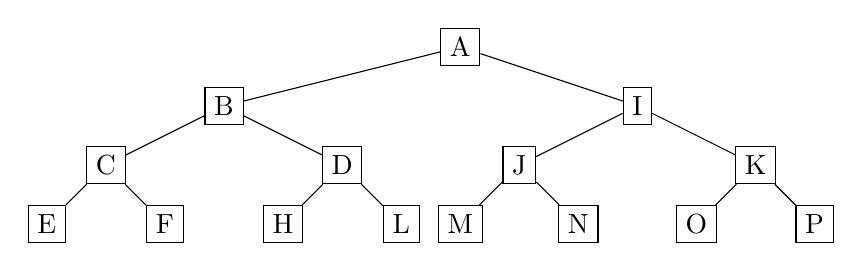
\begin{tikzpicture}[scale=0.75]
            \node[draw] (A) at (1,0) {A};
            \node[draw] (B) at (-3,-1) {B};
            \node[draw] (C) at (-5,-2) {C};
            \node[draw] (D) at (-1,-2) {D};
            \node[draw] (E) at (-6,-3) {E};
            \node[draw] (F) at (-4,-3) {F};
            \node[draw] (H) at (-2,-3) {H};
            \node[draw] (I) at (4,-1) {I};
            \node[draw] (J) at (2,-2) {J};
            \node[draw] (K) at (6,-2) {K};
            \node[draw] (L) at (0,-3) {L};
            \node[draw] (M) at (1,-3) {M};
            \node[draw] (N) at (3,-3) {N};
            \node[draw] (O) at (5,-3) {O};
            \node[draw] (P) at (7,-3) {P};

            \draw (A) -- (B);
            \draw (C) -- (B);
            \draw (C) -- (E);
            \draw (C) -- (F);
            \draw (D) -- (B);
            \draw (D) -- (H);
            \draw (A) -- (I);
            \draw (J) -- (I);
            \draw (I) -- (K);
            \draw (L) -- (D);
            \draw (J) -- (M);
            \draw (J) -- (N);
            \draw (K) -- (O);
            \draw (K) -- (P);
        \end{tikzpicture}
        \captionof{figure}{Un arbre binaire parfait}
        \label{arbre}
    \end{center}

    \begin{itemize}
        \item niveau 0: $2^0=1$ nœuds
        \item niveau 1: $2^1=2$ nœuds
        \item \dots
        \item niveau h: $2^h$ nœuds
    \end{itemize}
\begin{center}
    On double le nombre de nœuds à chaque niveau.
    
\end{center}

\end{frame}
\begin{frame}
    \frametitle{}

    Somme des premiers termes d'une suite géométrique: $$\sum_{k=0}^{h}{2^k}=u_0×\dfrac{1-q^{h+1}}{1-q}$$
$$\sum_{k=0}^{h}{2^k}=1×\dfrac{1-2^{h+1}}{1-2}$$
$$\sum_{k=0}^{h}{2^k}=2^{h+1}-1$$

\begin{center}
    La taille maximale est inférieure ou égale à $2^{h+1}-1$
\end{center}
\end{frame}
\begin{frame}
    \frametitle{}

    \begin{aretenir}[]
    $$h+1 \leqslant N \leqslant 2^{h+1}-1$$
    \end{aretenir}
    \begin{aretenir}[Remarque]
    

Si on définit la hauteur comme le nombre de nœuds maximum entre la racine et une feuille, on a: $$h \leqslant N \leqslant 2^{h}-1$$

    \end{aretenir}
\end{frame}
\end{document}